\section{Characteristics of Service Meshes}

\begin{figure*}
    \centering
    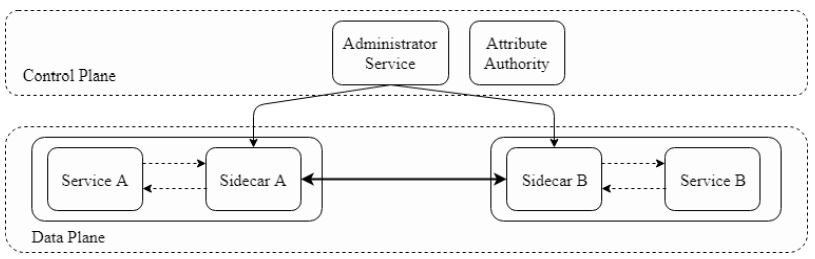
\includegraphics[width=0.8\textwidth]{img/mesh_detailed.JPG}
    \caption{Control and data plane in a service mesh\cite{sm4}}
    \label{fig:detailed mesh}
\end{figure*}

As mentioned in the previous chapter, creating an appropriate microservices infrastructure tend to be more complicated than implementing the business logic itself. For this reason, there is a need for infrastructure solutions that relieve the developers of the business logic. A service mesh is one conceivable solution approach and is defined as follows:

\subsection{Definition}

\begin{quote}
``A service mesh is a dedicated infrastructure layer for handling service-to-service communication. It’s responsible for the reliable delivery of requests through the complex topology of services that comprise a modern, cloud native application.
In practice, the service mesh is typically implemented as an array of lightweight network proxies that are deployed alongside application code, without the application needing to be aware." \cite[p. 123]{sm1}
\end{quote}

The last sentence of the definition sounds promising: The developer no longer has to worry about the infrastructure tasks. In the context of this paper, it should become clear how decoupled the infrastructure layer actually is.

\subsection{Architecture}

Figure \ref{fig:overview} shows a simplified microservice architecture using service meshes. The mentioned infrastructure layer is a composition of the lightweight network proxies, also called sidecards. These sidecars control the entire network communication between the microservice instances. Without service mesh, each service must implement this interservice logic on its own, which compromises developer focus on business goals. The figure perfectly illustrates that application services are decoupled from interservice communication.

\begin{figure}
    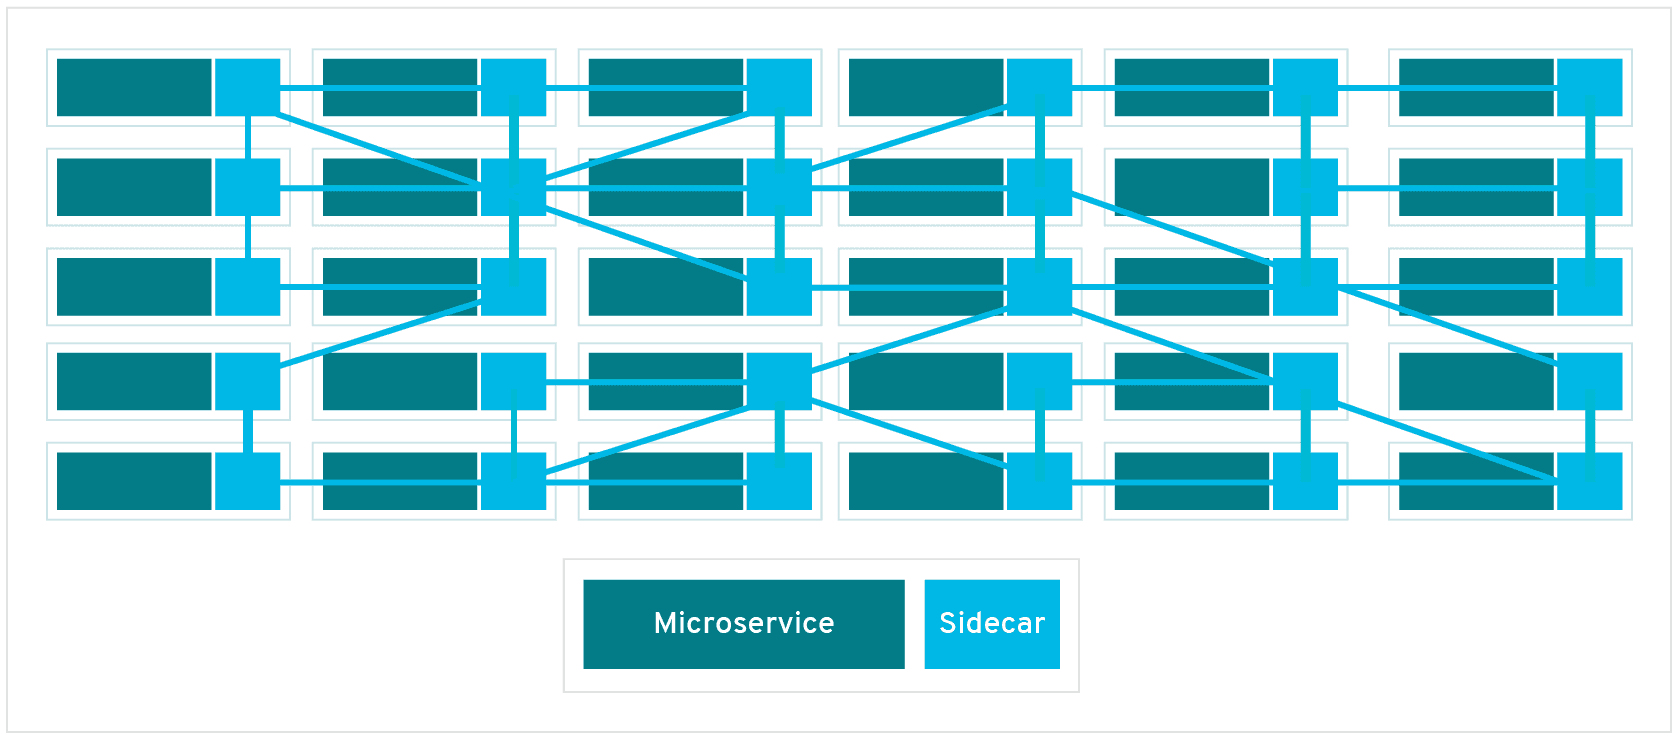
\includegraphics[width=\columnwidth]{img/mesh.png}
    \caption{Simplified service mesh based microservice architecture \cite{sm2}}
    \label{fig:overview}
\end{figure}

A more detailed illustration of a service mesh architecture is shown in figure \ref{fig:detailed mesh}. A service mesh consists of a control plane and a data plane.
The control plane is responsible for administrative tasks. This is where, for example, system-wide authentication and authorization policies are configured and made available to the proxies. Furthermore, settings for circuit breaking, timeouts and load balancing are made here. The composition of all application services with their sidecar proxies is called data plane \cite{sm4}.

\subsection{Central tasks}

Each service mesh has specific tasks to solve to enable microservice operation. These are named and briefly introduced below \cite{sm1}:

\subsubsection{Service discovery}

The number of service instances and the states and configurations change more frequently. For this reason, middleware is required to serve as an intermediary. It would be very complicated if every service A had to know under which IP and which port it can reach service B.

\subsubsection{Load balancing}

A load balancer is necessary to skillfully distribute requests to a service among replicas when loads are higher.

\subsubsection{Fault tolerance}

The microservice application must not be overly dependent on individual replicas being in a faulty state. For this reason, the service mesh must solve the task of forwarding requests only to services that have a sufficient health state.

\subsubsection{Traffic monitoring}

All communication between all microservices must be recorded and made visible, for example, via a central dashboard. In addition to logging, it makes sense to display metrics and statistics for the individual services.

\subsubsection{Circuit breaking}
Microservices need to be resilient. One way to do this is to implement the circuit breaker pattern. If recurring connection errors are detected for a resource, access to this resource is blocked by the circuit breaker so that it is not overloaded further.

\subsubsection{Authentication and access control}

With the use of a service mesh, it should be easy to apply and remove certain policies for authentication and authorization. One such policy could be that access to Service A, which provides the database logic, is only allowed by Service B and no one else.

\subsection{Opportunities and risks}

\begin{figure}
    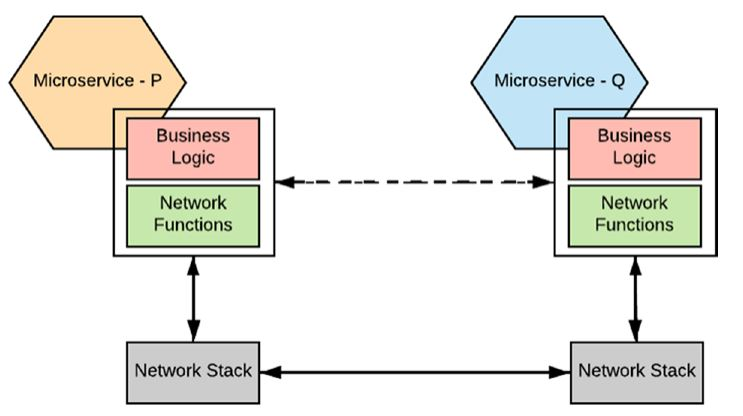
\includegraphics[width=\columnwidth]{img/microservices_without_mesh.JPG}
    \caption{Ex. architecture of microservices without service mesh\cite[S. 265]{sm4}}
    \label{fig:microservice-without-mesh}
\end{figure}


To highlight the benefits of a services mesh, you need to imagine a microservice architecture without services meshes. Figure 4 illustrates that each microservice requires a significant amount of logic to enable interservice communication. The effort required to implement this logic multiplies if, for example, Circuit Breaker is required in Java, Node JS, and Python. Since the requirements for infrastructure logic are the same in almost all microservice applications, it only makes sense to map this logic to an abstracted layer. This is where the service mesh comes into play. According to \cite{sm4}, the further advantages and drawbacks of a service mesh are as follows:

\subsubsection{Advantages}

\begin{itemize}

    \item Developers can concentrate on implementing their business applications. The management of a service mesh is more the task of an administrator or DevOps engineer.

    \item Polyglot support is another key benefit of service meshes. Developers can use their favorite programming languages and frameworks.

    \item In addition, the monitoring of services works out of the box. Distributed tracing and metrics require no additional effort from the developer's perspective. Furthermore, the application is decentralized, but centrally maintainable through the control plane. 

\end{itemize}
\subsubsection{Drawbacks}

\begin{itemize}
    \item On the other hand, service meshes also have disadvantages. Of course, the complexity of the architecture increases significantly by adding a sidecar proxy to each service instance. This also leads to the fact that each service call requires an additional hop.
    \item In addition, there are some problems in inter-service communication that service meshes do not address. These include complex routing, type mapping, and integration of other services and systems.
    \item A final important point is that service meshes are a comparatively new technology. The solutions are not necessarily mature enough for highly scaling environments.
\end{itemize}







